\section{Μεθοδολογία και περιβάλλον πειραμάτων}
Η αξιολόγηση οργανώθηκε ώστε κάθε συμπέρασμα να συνδέεται με συγκεκριμένη
μέτρηση ή λειτουργικό τεκμήριο. Ως περιβάλλον
αναφοράς χρησιμοποιείται EC2 instance τύπου \texttt{t3.small} στην περιοχή
\texttt{eu-central-1}, με Amazon Linux~2023 και EBS volume \texttt{gp3}
30~GiB. Στο instance εκτελούνται τρία Docker containers: Nginx, Spring Boot
και MySQL~8.4. Το Nginx αποτελεί το μοναδικό δημόσιο σημείο εισόδου στις
θύρες 80 και 443, ενώ η βάση δεδομένων παραμένει στο εσωτερικό δίκτυο της
εγκατάστασης.

Για να είναι συγκρίσιμα τα πειράματα, κάθε βαθμίδα φόρτου χρησιμοποίησε την
ίδια έκδοση εφαρμογής, σταθερό συνθετικό σύνολο δεδομένων και κοινή αρχική
κατάσταση. Οι χρόνοι καταγράφηκαν σε UTC και τα αποτελέσματα εφαρμογής
συσχετίστηκαν με τα metrics του ίδιου χρονικού παραθύρου στο CloudWatch.
Η Εικόνα~\ref{fig:experimental-workflow} συνοψίζει τη διαδικασία.

\begin{figure}[htbp]
\centering
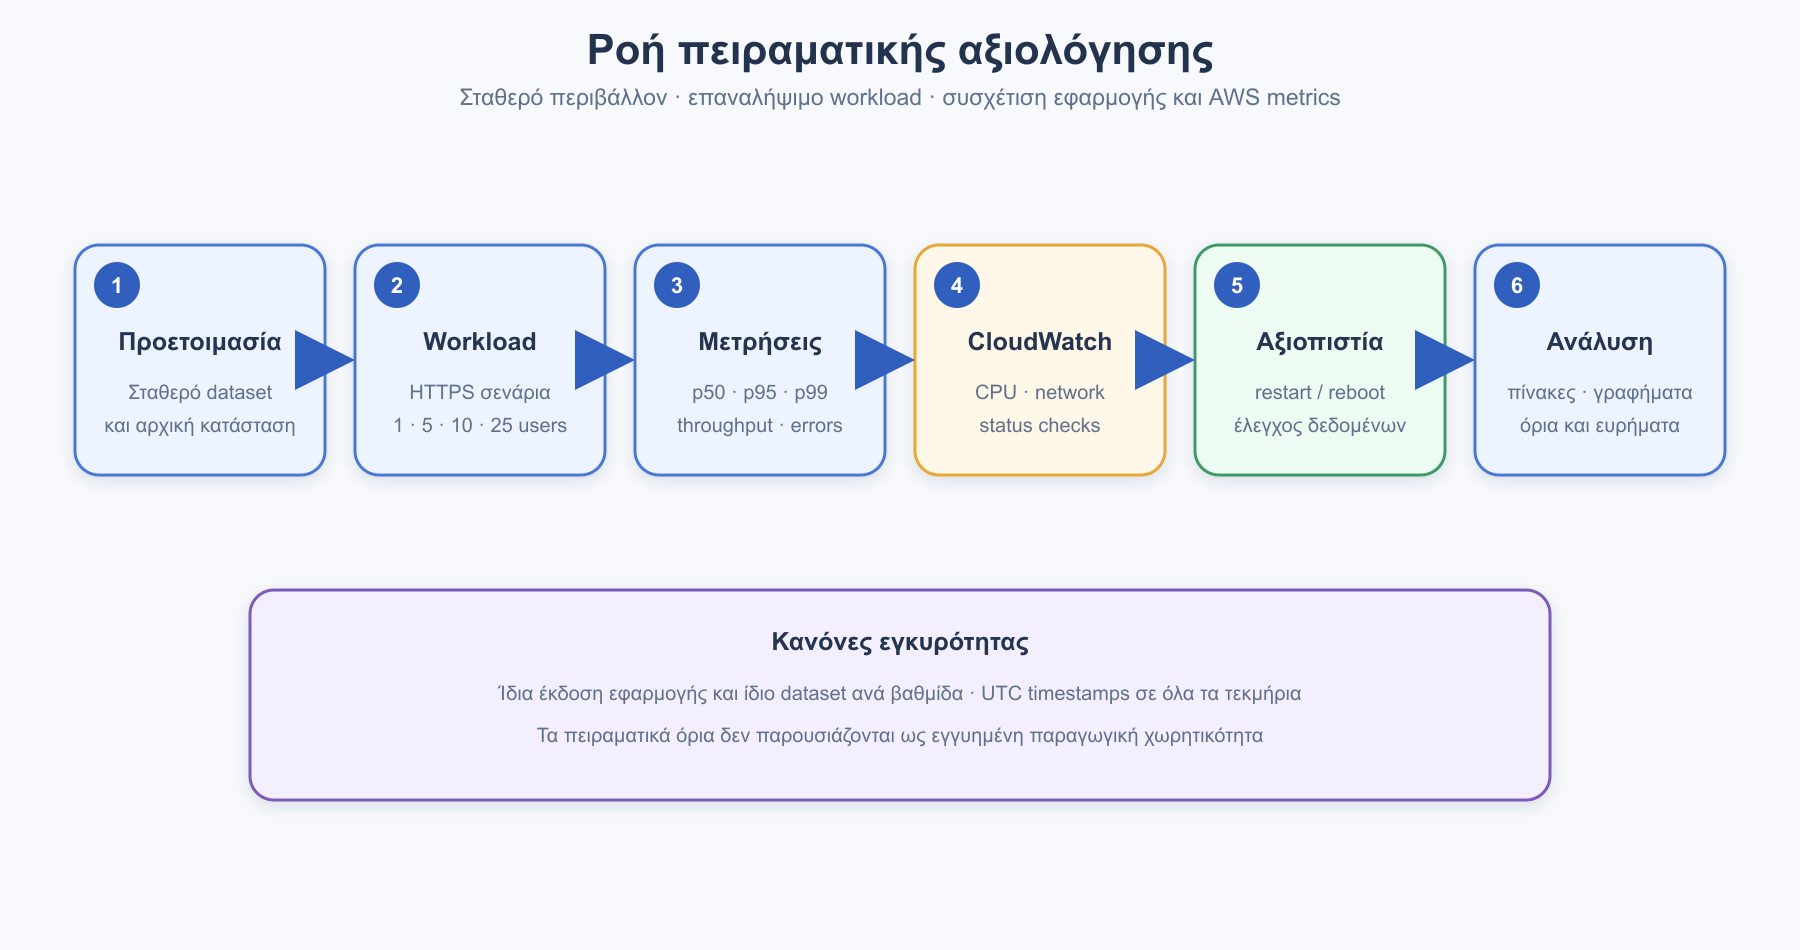
\includegraphics[width=\textwidth]{figures/evaluation/experimental-workflow.png}
\caption{Ροή πειραματικής αξιολόγησης από την προετοιμασία του σταθερού
dataset έως τη συσχέτιση των χρόνων απόκρισης, των AWS metrics και των
ελέγχων αξιοπιστίας.}
\label{fig:experimental-workflow}
\end{figure}

Οι μεταβλητές που καταγράφηκαν είναι ο αριθμός αιτημάτων, το throughput
(ρυθμός ολοκλήρωσης επιτυχών αιτημάτων ανά δευτερόλεπτο), το ποσοστό
σφαλμάτων, οι χρόνοι απόκρισης p50, p95 και p99, καθώς και CPU, network
traffic και status checks του EC2. Τα p50, p95 και p99 είναι εκατοστημόρια
(percentiles) και όχι ποσοστά καθυστέρησης: p50 είναι η διάμεσος, ενώ p95
σημαίνει ότι το 95\% των αποκρίσεων ολοκληρώθηκε σε χρόνο μικρότερο ή ίσο
από την αναφερόμενη τιμή και το βραδύτερο 5\% χρειάστηκε περισσότερο χρόνο.
Αντίστοιχα, το p99 καλύπτει το 99\% και απομονώνει το βραδύτερο 1\% των
παρατηρήσεων. Τα εκατοστημόρια είναι χρησιμότερα από έναν μεμονωμένο μέσο
όρο όταν λίγες πολύ αργές αποκρίσεις δημιουργούν ουρά καθυστέρησης
\cite{grafana2026k6metrics,grafana2026k6thresholds}.

Η μνήμη του application container καταγράφηκε με στιγμιότυπα του Docker και
όχι ως βασικό EC2 metric, επειδή δεν είχε εγκατασταθεί CloudWatch Agent.
Κάθε αριθμητικό αποτέλεσμα συνοδεύεται από διάρκεια, βαθμίδα ταυτόχρονων
χρηστών και ακριβές χρονικό παράθυρο.

\section{Λειτουργική επαλήθευση}
Οι λειτουργικοί έλεγχοι πραγματοποιήθηκαν στην παραγωγική εγκατάσταση με
συνθετικά δεδομένα. Μετά την ενεργοποίηση του Docker, τα containers της
εφαρμογής και του Nginx βρέθηκαν σε κατάσταση λειτουργίας, ενώ η MySQL πέρασε
τον ενσωματωμένο έλεγχο υγείας. Τα root και \texttt{www} DNS names επιλύθηκαν
στην ίδια Elastic IP, η διαδρομή HTTP επέστρεψε μόνιμη ανακατεύθυνση 301 και
η τελική διαδρομή HTTPS επέστρεψε 200 με έγκυρο πιστοποιητικό.

Η ροή νέου λογαριασμού επαληθεύτηκε από άκρο σε άκρο: υποβολή εγγραφής,
παράδοση email μέσω Amazon SES, επιβεβαίωση διεύθυνσης, απόρριψη σύνδεσης όσο
ο λογαριασμός παρέμενε ανενεργός, έγκριση από administrator και επιτυχής
είσοδος. Με την ίδια υποδομή email επαληθεύτηκε η αίτηση επαναφοράς κωδικού,
η παραλαβή συνδέσμου, η επιλογή νέου κωδικού και η επιτυχής μεταγενέστερη
σύνδεση.

Ελέγχθηκε επίσης η ασφαλής διαγραφή λογαριασμών προσωπικού. Τέσσερα
αυτοματοποιημένα tests επιβεβαίωσαν τη διαγραφή απλού προσωπικού και ιδιοκτήτη
κλινικής χωρίς ραντεβού, την προστασία του \texttt{SUPERADMIN} και την
απόρριψη με HTTP~409 όταν υπάρχουν συνδεδεμένες εγγραφές ραντεβού.

Η production σελίδα \enquote{Profile \& Integrations} επαληθεύτηκε επίσης
ως προσβάσιμη τόσο από τη διαδρομή \texttt{/profile} όσο και από την κάρτα
του συνδεδεμένου χρήστη στην πλευρική πλοήγηση. Εμφάνισε ανεξάρτητα τα
στοιχεία επικοινωνίας και την κατάσταση Google Calendar, ενώ η επιλογή
\enquote{Connect Google Calendar} οδήγησε επιτυχώς στην πραγματική οθόνη
συγκατάθεσης της Google για τον μοναδικό OAuth test user. Κατά την πρώτη
δοκιμή εντοπίστηκε αστοχία στη διαδρομή επιστροφής: ένα παρωχημένο ή
αντικατεστημένο \texttt{state} παρήγαγε \texttt{reason=invalid} και η σελίδα
αποτελέσματος προστατευόταν λανθασμένα, με συνέπεια HTTP~401. Η διόρθωση
κατέστησε δημόσια μόνο τη σελίδα αποτελέσματος, διατήρησε προστατευμένο το
profile, όρισε ρητά ασφαλή χαρακτηριστικά στο session cookie και πρόσθεσε
καταγραφή των αποτυχιών ελέγχου \texttt{state}. Η διόρθωση αναπτύχθηκε στην
παραγωγή και επαληθεύτηκε με επιτυχή εκκίνηση του Spring container, παρουσία
των μεταβλητών Google και απόκριση HTTPS~200. Η διαδρομή αποτελέσματος
ελέγχθηκε επίσης άμεσα και επέστρεψε HTTP~200 αντί του προηγούμενου 401. Η
εξουσιοδότηση του λογαριασμού administrator ολοκληρώθηκε και δύο υπάρχοντα
ραντεβού δημιουργήθηκαν στο Google Calendar. Η πρώτη οπτική σύγκριση ανέδειξε
μετατόπιση τριών ωρών: ώρες 11:00 και 12:00 της εφαρμογής εμφανίστηκαν ως
14:00 και 15:00, επειδή το container χρησιμοποιούσε UTC για τοπικές τιμές.
Η μετατροπή διορθώθηκε ώστε να χρησιμοποιεί ρητά τη ζώνη
\texttt{Europe/Athens} και αναπτύχθηκε εκ νέου στην παραγωγή. Στην επανάληψη
του ελέγχου, το ενημερωμένο ραντεβού εμφανίστηκε στις 09:30 τόσο στο Happy
Tails όσο και στο Google Calendar, ενώ η πρόσκληση email ανέφερε 09:30--10:00
και Eastern European Time--Athens. Η διαγραφή αφαίρεσε το απομακρυσμένο event
και το Google Calendar παρήγαγε την αντίστοιχη ειδοποίηση ακύρωσης. Το
συγκεκριμένο τεκμήριο αφορά το κανάλι Google και όχι μήνυμα από τον
\texttt{no-reply} sender του Amazon SES. Έτσι επαληθεύτηκαν οι ροές create, update
και delete μαζί με τη σωστή μετατροπή ζώνης ώρας.
Στο συγκεκριμένο test ο administrator/organizer και η client owner
χρησιμοποίησαν διαφορετικές διευθύνσεις και ανεξάρτητες θυρίδες email.
Επομένως επαληθεύτηκε τόσο η παραγωγή των role-based παραληπτών όσο και η
παράδοση της πρόσκλησης σε διακριτό παραλήπτη ιδιοκτήτη.

Στον ιατρικό φάκελο μεταφορτώθηκε τυχαίο PDF, μη συνδεδεμένο με πραγματικό
περιστατικό. Η εφαρμογή αποθήκευσε τα metadata και εμφάνισε ενεργή ενέργεια
\enquote{Προβολή}. Η επιλογή της ενέργειας ανέκτησε και εμφάνισε επιτυχώς το
PDF στον browser. Το περιεχόμενο του παραστατικού δεν χρησιμοποιείται ως
δεδομένο της μελέτης και δεν παρουσιάζεται στη διατριβή.

\begin{table}[htbp]
\centering
\caption{Συνοπτικά αποτελέσματα λειτουργικής επαλήθευσης.}
\label{tab:functional-verification}
\small
\begin{tabularx}{\textwidth}{p{0.28\textwidth}X p{0.18\textwidth}}
\toprule
Έλεγχος & Παρατηρηθέν αποτέλεσμα & Κατάσταση \\
\midrule
Docker services & Spring Boot και Nginx σε λειτουργία, MySQL healthy & Επιτυχία \\
DNS και TLS & Root/\texttt{www} στην Elastic IP, HTTP 301, HTTPS 200 & Επιτυχία \\
Εγγραφή χρήστη & SES email, verification, διοικητική έγκριση, login & Επιτυχία \\
Επαναφορά κωδικού & Email reset, αλλαγή κωδικού και νέα είσοδος & Επιτυχία \\
Διαγραφή λογαριασμού προσωπικού & Επιτυχία για μη χρησιμοποιούμενο λογαριασμό, προστασία \texttt{SUPERADMIN} και HTTP~409 όταν υπάρχουν ραντεβού & Επιτυχία \\
Μεταφόρτωση PDF & Αποθήκευση metadata και αρχείου περίπου 1,1~MB & Επιτυχία \\
Προβολή PDF & Ανάκτηση και εμφάνιση μέσω \enquote{Προβολή} & Επιτυχία \\
Liquibase startup & 4 previously run, 0 νέα changesets, lock released & Επιτυχία \\
Profile και OAuth consent & Πρόσβαση από user card, συγκατάθεση και σύνδεση administrator Calendar & Επιτυχία \\
Google event create/update & Ίδιο event στις 09:30 σε εφαρμογή, Google Calendar και πρόσκληση Athens & Επιτυχία \\
Google event delete & Αφαίρεση απομακρυσμένου event και παραλαβή ειδοποίησης ακύρωσης & Επιτυχία \\
\bottomrule
\end{tabularx}
\end{table}

\section{Περιορισμένο proof of concept με Amazon CloudFront}
Δημιουργήθηκε ξεχωριστή CloudFront distribution με όνομα
\path{happy-tails-thesis-poc}, σύμφωνα με τις παραμέτρους διανομής που
τεκμηριώνει η AWS~\cite{aws2026cloudfront}. Ως custom origin ορίστηκε το
υφιστάμενο HTTPS endpoint \texttt{thesis-tasiopoulos.com}. Δεν ορίστηκε
alternate domain name και δεν τροποποιήθηκαν οι εγγραφές Route~53· επομένως
η παραγωγική διαδρομή παρέμεινε ανεξάρτητη από το πείραμα. Η πρόσβαση στη
δοκιμή έγινε αποκλειστικά από το προεπιλεγμένο hostname
\path{dkaqy32zt0b9h.cloudfront.net}.

Επειδή η εφαρμογή είναι δυναμική και χρησιμοποιεί authenticated API calls,
η προεπιλεγμένη συμπεριφορά ρυθμίστηκε με \texttt{CachingDisabled}, με
origin request policy \path{AllViewerExceptHostHeader}. Με αυτόν τον τρόπο
προωθούνται cookies, query strings και viewer headers, αλλά το \texttt{Host}
προσαρμόζεται στο origin ώστε να συμφωνεί με το πιστοποιητικό TLS του
\texttt{thesis-tasiopoulos.com}. Επιτράπηκαν οι μέθοδοι \texttt{GET},
\texttt{HEAD}, \texttt{OPTIONS}, \texttt{PUT}, \texttt{POST}, \texttt{PATCH}
και \texttt{DELETE}, ενώ τόσο η σύνδεση viewer--CloudFront όσο και η σύνδεση
CloudFront--origin προστατεύονται με HTTPS. Οι ενσωματωμένες προστασίες WAF
του plan ενεργοποιήθηκαν σε monitor mode, ώστε το πείραμα να παρατηρεί
αιτήματα χωρίς να παρεμβαίνει στη λειτουργία τους.

Η λειτουργική επαλήθευση έδειξε ότι η δημόσια αρχική σελίδα και η διαδρομή
\texttt{/login} φορτώθηκαν επιτυχώς μέσω του CloudFront hostname. Επιπλέον,
αίτημα προς την HTTP εκδοχή του hostname ανακατευθύνθηκε αυτόματα σε HTTPS.
Οι έλεγχοι αυτοί τεκμηριώνουν τη βασική συνδεσιμότητα και τη δρομολόγηση, όχι
όμως βελτίωση απόδοσης, διότι το caching παρέμεινε σκόπιμα απενεργοποιημένο
και δεν έχει ακόμη εκτελεστεί συγκριτικό workload.

\section{Αξιολόγηση απόδοσης και χρόνου απόκρισης}
Η αρχική μέτρηση χρόνου απόκρισης κάλυψε τόσο τη δημόσια αρχική σελίδα όσο
και αυθεντικοποιημένες λειτουργίες. Πριν από τη μέτρηση αναπτύχθηκε και
επαληθεύτηκε πανομοιότυπο artifact με SHA-256
\texttt{317132aeac05\ldots 2153c82f3}. Χρησιμοποιήθηκε απομονωμένος
συνθετικός λογαριασμός με αποκλειστικά τον ρόλο \texttt{STAFF}, χωρίς
συσχέτιση με πραγματικό πρόσωπο, κτηνίατρο, Google Calendar ή πραγματική
διεύθυνση email. Ο κωδικός δημιουργήθηκε τυχαία για το πείραμα και δεν
καταγράφηκε στο αποτέλεσμα.

Μετά από πέντε αιτήματα warm-up, δηλαδή προκαταρκτικά αιτήματα για την
αρχικοποίηση συνδέσεων και runtime paths πριν από τη μέτρηση, ένας εικονικός
χρήστης (Virtual User, VU) πραγματοποίησε για
60,04~s κυκλικά αιτήματα προς τη δημόσια αρχική σελίδα και τα
\texttt{GET /api/dashboard}, \texttt{GET /api/owners} και
\texttt{GET /api/appointments}. Η αυθεντικοποίηση εκτελέστηκε μία φορά στην
αρχή μέσω \texttt{POST /api/auth/login}. Το ακριβές παράθυρο ήταν
2026-09-05 13:19:08,191 έως 13:20:08,220~UTC. Καταγράφηκαν 895 αιτήματα με
895 επιτυχίες, μηδενικά σφάλματα και συνολικό throughput 14,91
αιτήματα/s. Τα αποτελέσματα ανά endpoint παρουσιάζονται στον
Πίνακα~\ref{tab:baseline-response-times}.

\begin{table}[htbp]
\centering
\caption{Χρόνοι απόκρισης του baseline με έναν εικονικό χρήστη.}
\label{tab:baseline-response-times}
\small
\setlength{\tabcolsep}{4pt}
\begin{tabularx}{\textwidth}{>{\raggedright\arraybackslash}X r r r r r}
\toprule
Endpoint & Αιτήματα & p50 (ms) & p95 (ms) & p99 (ms) & Σφάλματα \\
\midrule
\path{POST /api/auth/login} & 1 & 429,53 & 429,53 & 429,53 & 0 \\
\texttt{GET /} & 223 & 59,97 & 67,87 & 355,49 & 0 \\
\path{GET /api/dashboard} & 224 & 58,06 & 83,35 & 141,20 & 0 \\
\path{GET /api/owners} & 224 & 69,19 & 91,85 & 108,70 & 0 \\
\path{GET /api/appointments} & 223 & 64,03 & 77,20 & 93,66 & 0 \\
\bottomrule
\end{tabularx}
\end{table}

Η μοναδική μέτρηση login δεν αποτελεί κατανομή και παρατίθεται μόνο ως
χρόνος αρχικοποίησης. Στα επαναλαμβανόμενα endpoints, το υψηλότερο p95 ήταν
91,85~ms στη λίστα ιδιοκτητών. Το p99 της αρχικής σελίδας έφθασε τα
355,49~ms, παρότι το p95 παρέμεινε 67,87~ms, γεγονός που δείχνει λίγες
μεμονωμένες αργές αποκρίσεις και δικαιολογεί τη χρήση percentiles αντί ενός
μόνο μέσου όρου. Δεν καταγράφηκαν \texttt{ERROR}, exception ή
\texttt{OutOfMemory} μηνύματα στο Spring container κατά το ίδιο παράθυρο,
ενώ ο έλεγχος μετά τη δοκιμή επέστρεψε HTTPS~200.

Τα βασικά EC2 metrics του CloudWatch συσχετίστηκαν με τα δύο πεντάλεπτα
διαστήματα που τέμνουν το workload. Στο διάστημα 13:15--13:20~UTC η μέση και
μέγιστη CPU ήταν 3,10\% και 10,20\%, με 335.554 bytes εισόδου και 1.080.736
bytes εξόδου. Στο διάστημα 13:20--13:25~UTC οι διαθέσιμες κατά τη συλλογή
τιμές ήταν 8,85\% μέση και 16,25\% μέγιστη CPU, 102.778 bytes εισόδου και
311.303 bytes εξόδου. Το \texttt{StatusCheckFailed} ήταν μηδέν και στα δύο
διαστήματα. Επειδή η δοκιμή διήρκεσε ένα λεπτό και διέσχισε το όριο των
13:20, τα πεντάλεπτα metrics αποτελούν συσχετισμένα και όχι αποκλειστικά
αποδιδόμενα δείγματα του workload.

\section{Δοκιμές φόρτου και χρήσης πόρων}
Η δοκιμή φόρτου εκτελέστηκε σε βαθμίδες 1, 5, 10 και 25 ταυτόχρονων
εικονικών χρηστών (VU). Κάθε VU εκτελεί ανεξάρτητα το ίδιο σενάριο και
προσομοιώνει έναν ενεργό χρήστη· δεν ισοδυναμεί με ένα μόνο αίτημα, διότι
μπορεί να ολοκληρώσει πολλά διαδοχικά αιτήματα στη διάρκεια της δοκιμής
\cite{grafana2026k6metrics}. Κάθε βαθμίδα είχε διάρκεια περίπου 60~s και την ίδια
κυκλική αναλογία των τεσσάρων λειτουργιών ανάγνωσης. Κάθε εικονικός χρήστης
πραγματοποίησε μία ανεξάρτητη αυθεντικοποίηση πριν από τον βρόχο αιτημάτων.
Οι τέσσερις βαθμίδες εκτελέστηκαν διαδοχικά μόνο όταν η προηγούμενη
ολοκληρωνόταν χωρίς σφάλματα και η εφαρμογή παρέμενε διαθέσιμη. Ο
Πίνακας~\ref{tab:load-stages} συνοψίζει τα αποτελέσματα.

\begin{table}[htbp]
\centering
\caption{Αποτελέσματα των διαδοχικών βαθμίδων φόρτου.}
\label{tab:load-stages}
\small
\begin{tabularx}{\textwidth}{r r r r r r X}
\toprule
VU & Αιτήματα & req/s & Σφάλματα & μέγ. read p95 & login p95 & Μνήμη app μετά \\
\midrule
1  & 895    & 14,91  & 0 & 91,85~ms  & 429,53~ms  & 399,3~MiB \\
5  & 4.803  & 79,77  & 0 & 87,28~ms  & 1.108,98~ms & 430,7~MiB \\
10 & 9.849  & 163,68 & 0 & 81,71~ms  & 2.049,57~ms & 477,1~MiB \\
25 & 20.480 & 339,73 & 0 & 109,72~ms & 7.710,72~ms & 571,6~MiB \\
\bottomrule
\end{tabularx}
\end{table}

Το throughput αυξήθηκε από 14,91 σε 339,73 αιτήματα/s και στη βαθμίδα των
25 χρηστών αντιστοιχούσε περίπου στο 91\% της απλής γραμμικής προβολής από
το baseline. Οι χρόνοι p95 των επαναλαμβανόμενων read endpoints παρέμειναν
κάτω από 110~ms σε όλες τις βαθμίδες και δεν παρουσιάστηκε αποτυχία.
Αντίθετα, το p95 της ταυτόχρονης αρχικής αυθεντικοποίησης αυξήθηκε από
429,53~ms σε 7,71~s στους 25 χρήστες. Η συμπεριφορά αυτή δείχνει ότι η
υπολογιστικά σκόπιμα ακριβή επαλήθευση BCrypt αποτελεί το πρώτο εμφανές
σημείο υποβάθμισης όταν πολλές νέες sessions αρχίζουν ταυτόχρονα. Στην ίδια
τελευταία βαθμίδα εμφανίστηκαν λίγες μέγιστες αποκρίσεις read έως 2,57~s,
παρότι το αντίστοιχο μέγιστο p99 ήταν 314,94~ms.

Η Εικόνα~\ref{fig:throughput-scaling} συγκρίνει το μετρημένο throughput με
την απλή γραμμική προβολή που προκύπτει από το baseline. Η
Εικόνα~\ref{fig:latency-p95-scaling} αποτυπώνει χωριστά τη συμπεριφορά του
login και των επαναλαμβανόμενων αναγνώσεων. Η δεύτερη σύγκριση είναι
ιδιαίτερα σημαντική, διότι δείχνει ότι το πρώτο όριο δεν βρίσκεται στα read
endpoints αλλά στην ταυτόχρονη επαλήθευση κωδικών.

\begin{figure}[htbp]
\centering
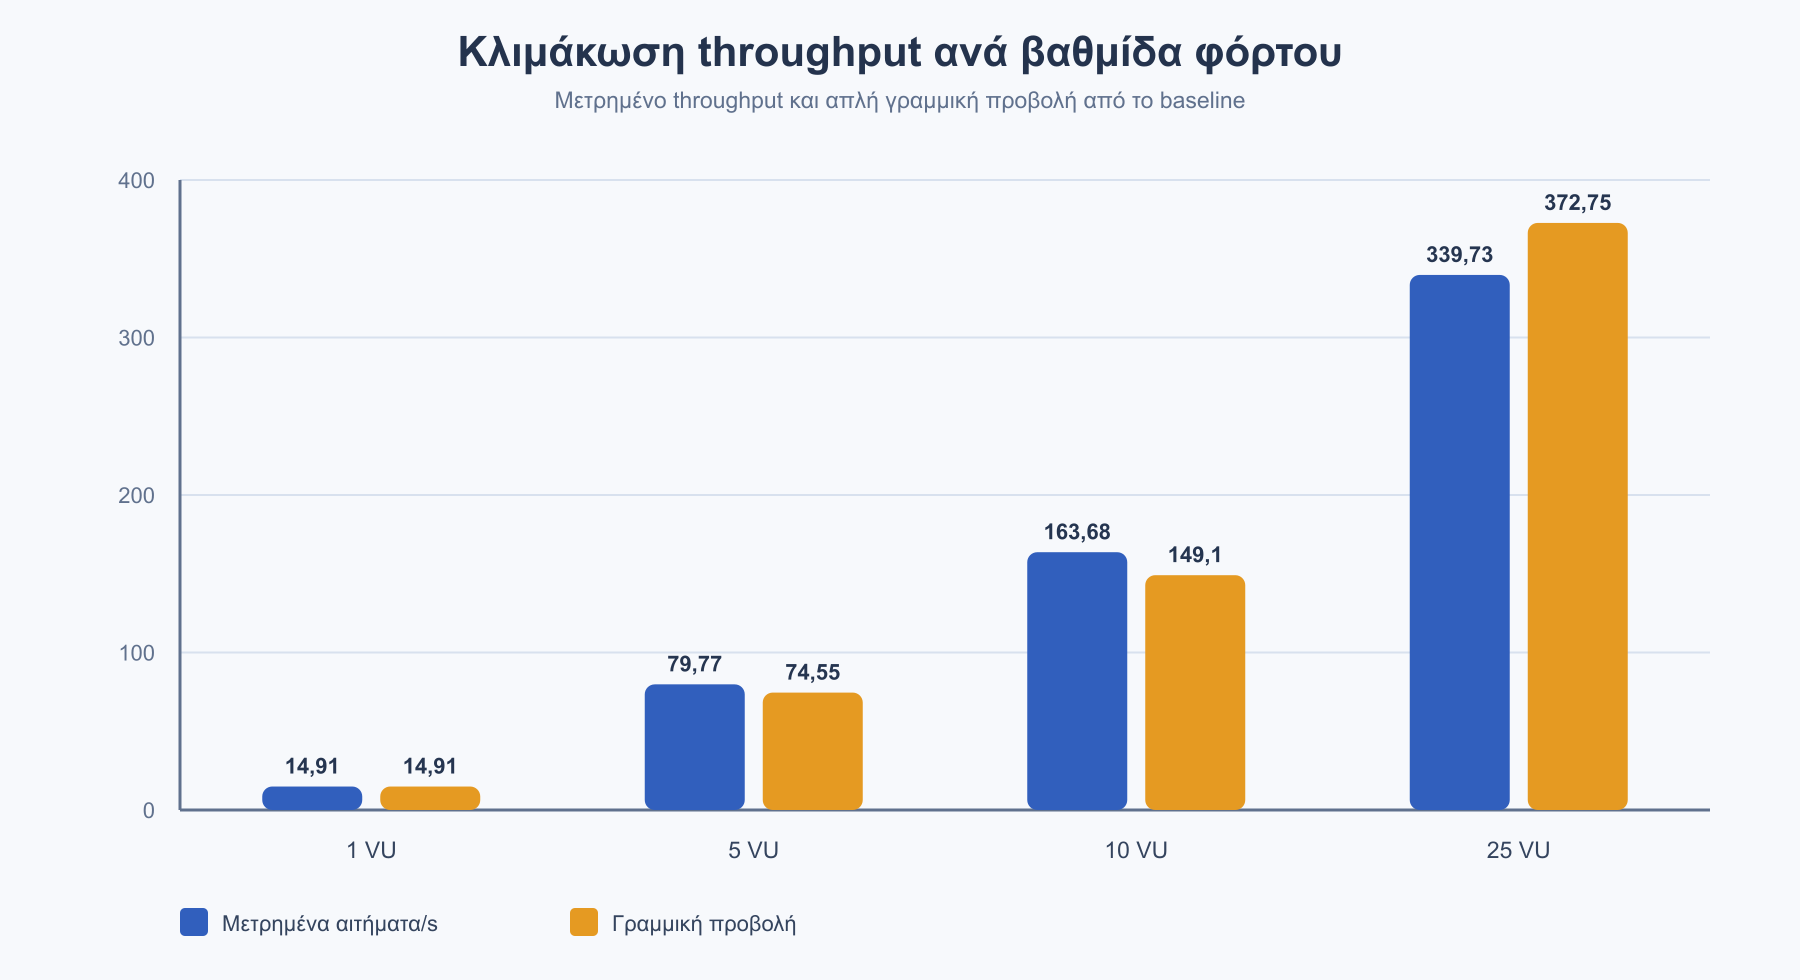
\includegraphics[width=\textwidth]{figures/evaluation/throughput-scaling.png}
\caption{Μετρημένο throughput ανά βαθμίδα φόρτου και σύγκριση με την απλή
γραμμική προβολή από το baseline.}
\label{fig:throughput-scaling}
\end{figure}

\begin{figure}[htbp]
\centering
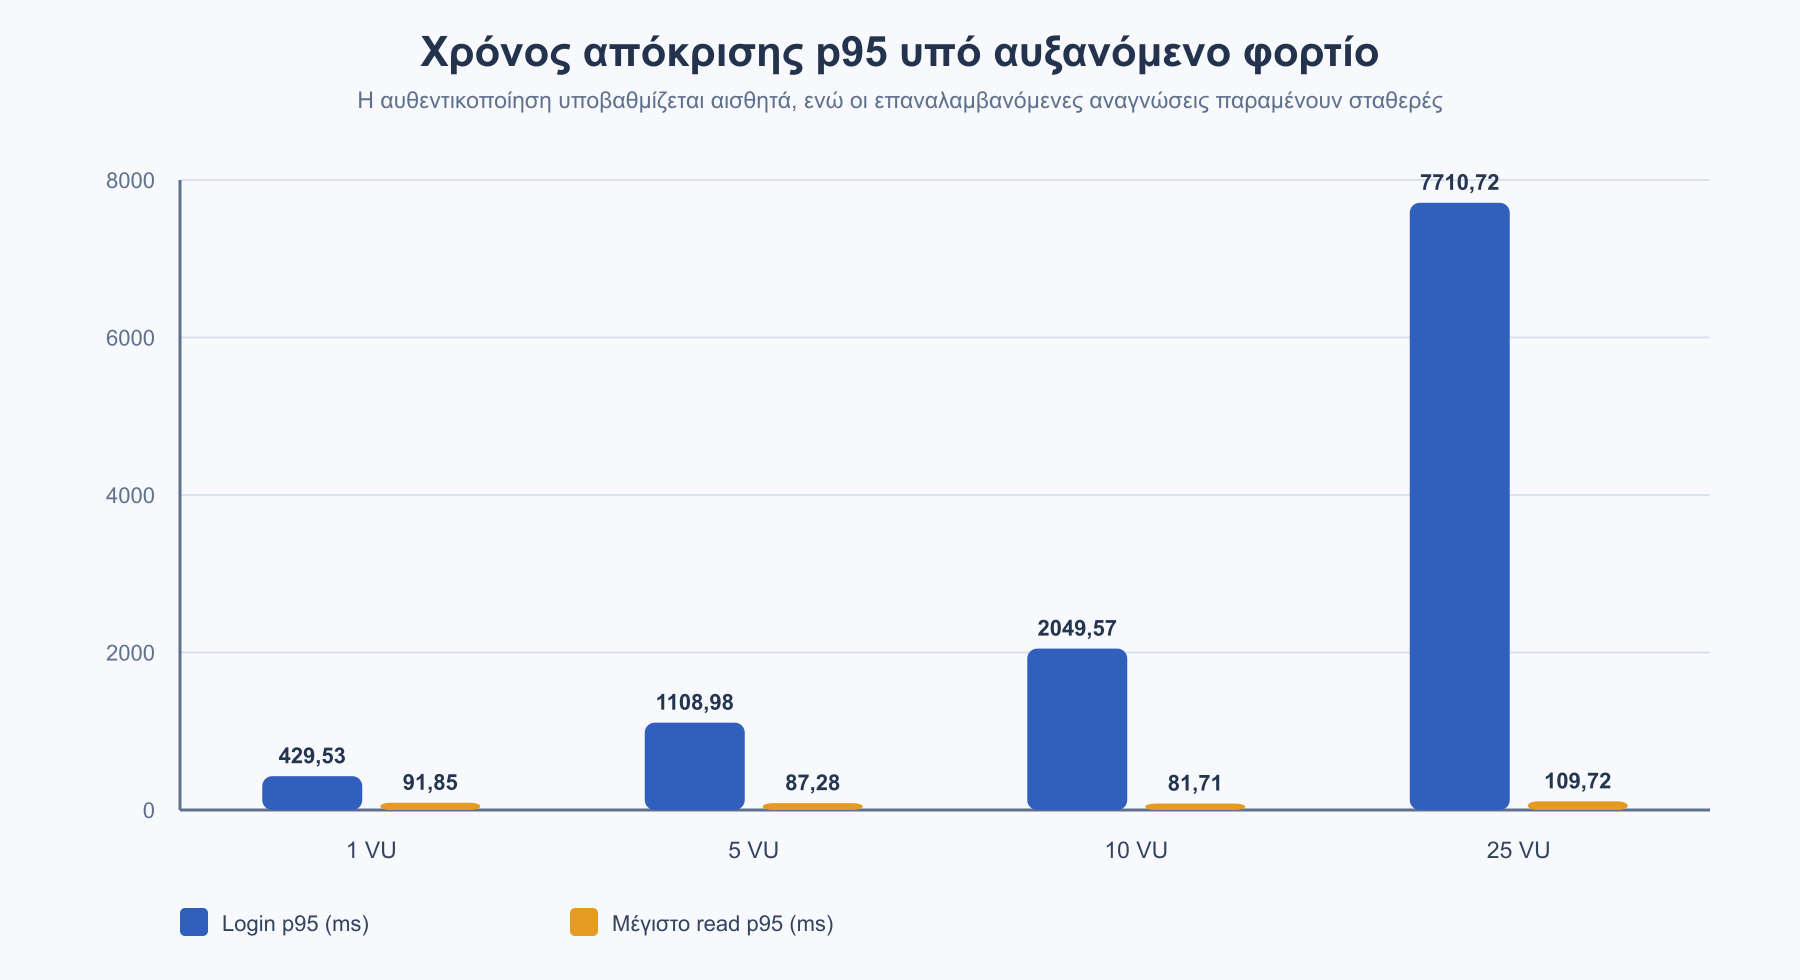
\includegraphics[width=\textwidth]{figures/evaluation/latency-p95-scaling.png}
\caption{Σύγκριση του p95 της αρχικής αυθεντικοποίησης με το υψηλότερο p95
των επαναλαμβανόμενων read endpoints ανά βαθμίδα φόρτου.}
\label{fig:latency-p95-scaling}
\end{figure}

Μετά από κάθε βαθμίδα, ο δημόσιος έλεγχος επέστρεψε HTTPS~200 και τα logs δεν
περιείχαν \texttt{ERROR}, exception ή \texttt{OutOfMemory}. Η στιγμιαία
χρήση μνήμης του Spring container αυξήθηκε από 399,3 σε 571,6~MiB, παραμένοντας
εντός του διαθέσιμου ορίου του instance. Στο πεντάλεπτο CloudWatch διάστημα
13:30--13:35~UTC, το οποίο περιλαμβάνει το τέλος της βαθμίδας των 10 χρηστών
και ολόκληρη τη βαθμίδα των 25, η μέση CPU ήταν 29,88\% και η μέγιστη
77,47\%. Καταγράφηκαν συνολικά 11.463.668 bytes εισόδου και 42.556.433 bytes
εξόδου, χωρίς αποτυχία status check. Επειδή οι σύντομες βαθμίδες τέμνουν τα
πεντάλεπτα aggregates και δύο από αυτές βρίσκονται στο ίδιο διάστημα, τα
metrics τεκμηριώνουν τη συνολική πίεση του high-load παραθύρου αλλά δεν
αποδίδονται αποκλειστικά σε μία βαθμίδα.

\begin{figure}[htbp]
\centering
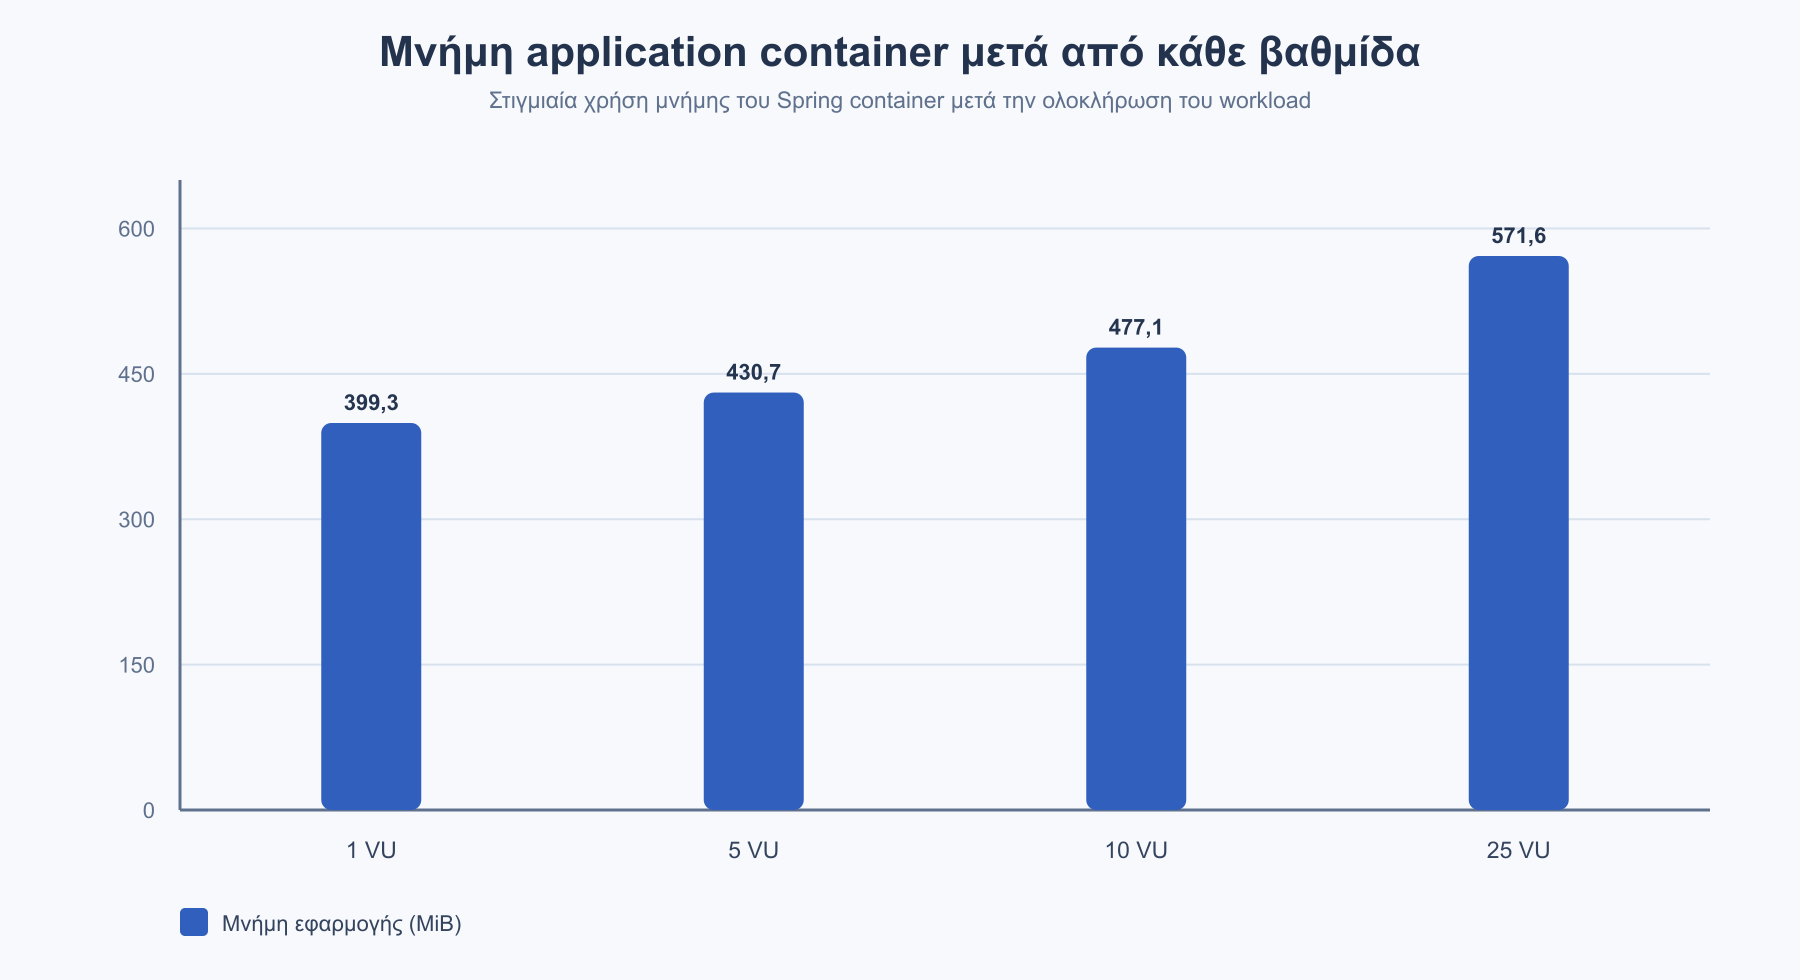
\includegraphics[width=\textwidth]{figures/evaluation/application-memory-scaling.png}
\caption{Στιγμιαία χρήση μνήμης του Spring container μετά από κάθε βαθμίδα
φόρτου. Οι τιμές αποτελούν μεταγενέστερα στιγμιότυπα και όχι μέγιστα της
ολόκληρης βαθμίδας.}
\label{fig:application-memory-scaling}
\end{figure}

Η βαθμίδα των 25 χρηστών χρησιμοποιήθηκε ως ελεγχόμενο stress endpoint και
εφαρμόστηκε το κριτήριο διακοπής: το login p95 είχε ήδη υπερβεί τα 7~s και η
μέγιστη CPU στο κοινό high-load παράθυρο έφθασε το 77,47\%. Η αύξηση πέρα
από αυτό το σημείο δεν ήταν αναγκαία για να αποδειχθεί η υποβάθμιση και θα
αύξανε άσκοπα τον κίνδυνο για τη μοναδική παραγωγική εγκατάσταση. Το όριο
αφορά το συγκεκριμένο πείραμα και δεν αποτελεί εγγυημένη παραγωγική
χωρητικότητα.

Στη συνέχεια εκτελέστηκε soak test πέντε εικονικών χρηστών για 300,29~s, από
13:36:51,714 έως 13:41:51,993~UTC. Ολοκληρώθηκαν 26.291 αιτήματα με
throughput 87,55 αιτήματα/s και μηδενικά σφάλματα. Τα p95 των τριών
αυθεντικοποιημένων read endpoints ήταν 64,16--67,65~ms και το μεγαλύτερο p95
όλων των reads ήταν 89,70~ms. Δεν παρατηρήθηκε χρονική αύξηση καθυστέρησης ή
αποτυχία διαθεσιμότητας. Σε ενδιάμεσο στιγμιότυπο το Spring container
χρησιμοποιούσε 570,9~MiB και 33,37\% CPU, ενώ η MySQL 499,8~MiB και 11,94\%
CPU.

Τα δύο πλήρη CloudWatch διαστήματα 13:35--13:40 και 13:40--13:45~UTC είχαν
μέση CPU 12,13\% και 12,57\%, μέγιστη 22,78\% και 23,43\% αντίστοιχα και
μηδενικό \texttt{StatusCheckFailed}. Συνολικά κατέγραψαν 10.854.409 bytes
εισόδου και 40.048.829 bytes εξόδου. Τα διαστήματα περιλαμβάνουν μικρό χρόνο
ηρεμίας πριν και μετά το πεντάλεπτο workload, αλλά δεν περιλαμβάνουν άλλη
δοκιμή φόρτου και παρέχουν καθαρότερη ένδειξη σταθερής χρήσης πόρων από τις
σύντομες βαθμίδες.

Η Εικόνα~\ref{fig:cloudwatch-cpu-windows} παρουσιάζει συγκεντρωτικά τη μέση
και τη μέγιστη CPU των πεντάλεπτων παραθύρων. Η κορύφωση στο διάστημα
13:30--13:35~UTC συμπίπτει με το τέλος της βαθμίδας των 10 χρηστών και τη
βαθμίδα των 25 χρηστών, ενώ τα δύο επόμενα παράθυρα αντιστοιχούν κυρίως στο
σταθερό soak workload. Η μέγιστη τιμή 77,47\% αποτελεί σύντομη αιχμή και όχι
παρατεταμένο κορεσμό του επεξεργαστή: η μέση τιμή του ίδιου παραθύρου ήταν
29,88\% και στα επόμενα δύο παράθυρα η μέγιστη χρήση υποχώρησε κάτω από
24\%. Ωστόσο, η αιχμή δείχνει ότι το διαθέσιμο περιθώριο CPU μειώνεται αισθητά
όταν αυξάνεται η ταυτόχρονη δραστηριότητα.

\begin{figure}[htbp]
\centering
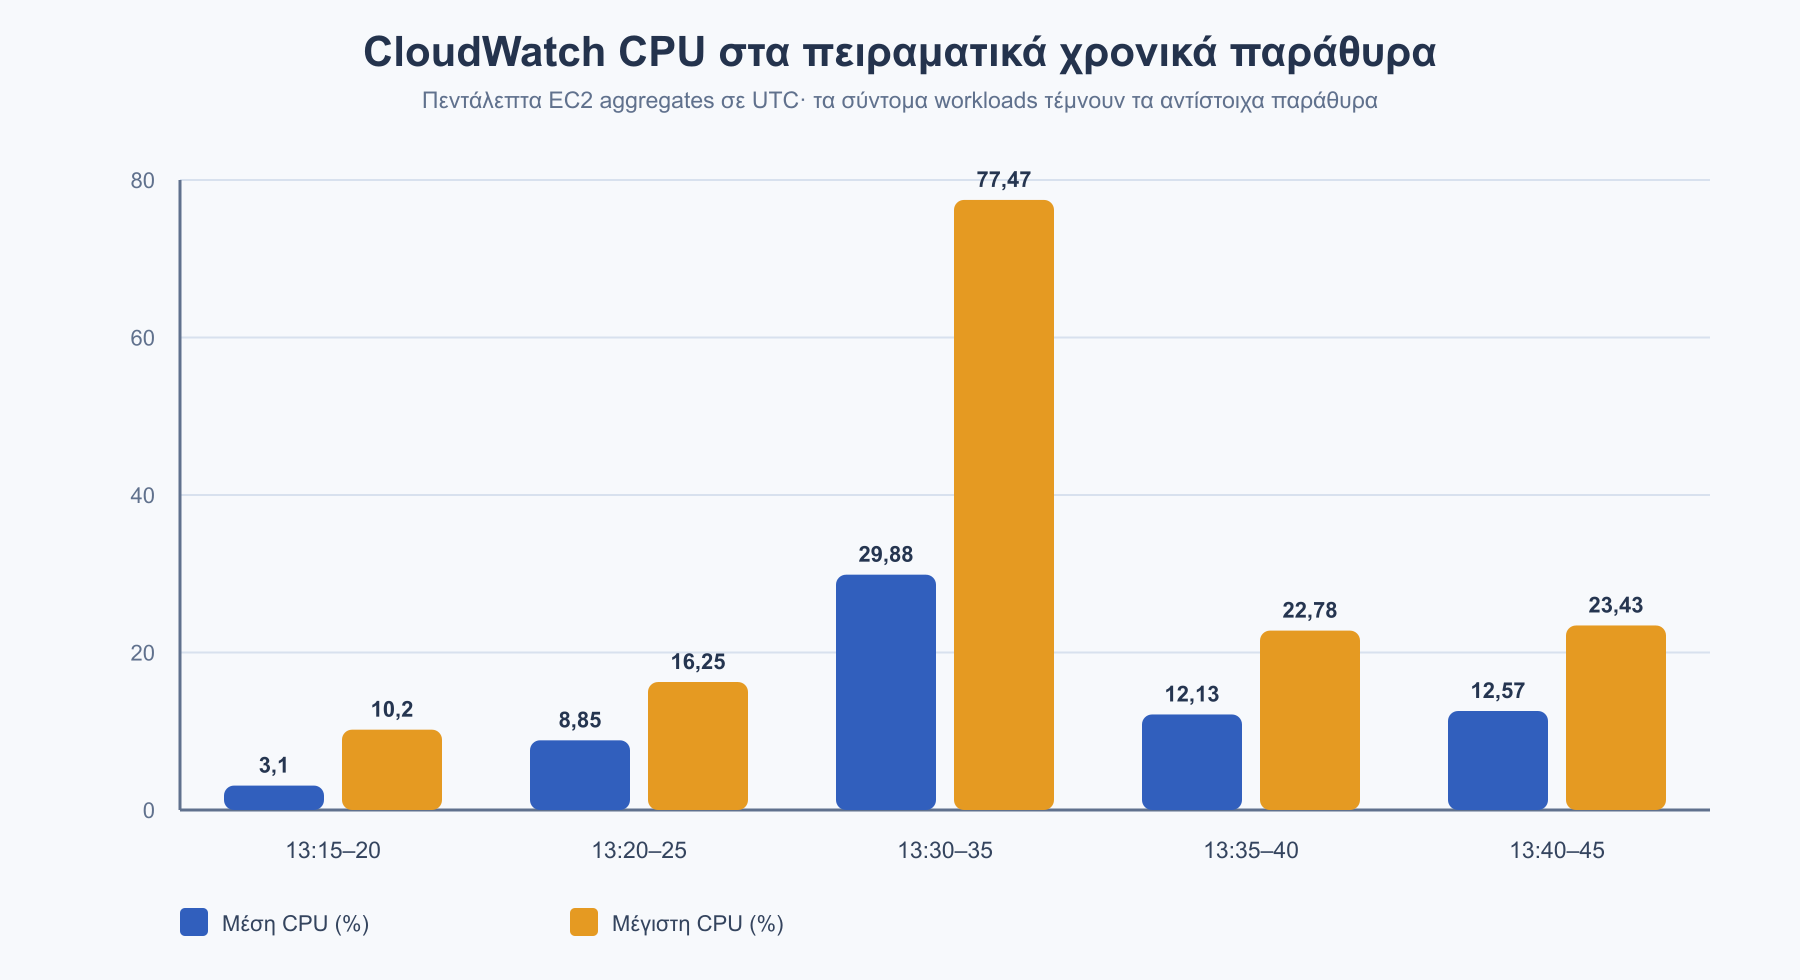
\includegraphics[width=\textwidth]{figures/evaluation/cloudwatch-cpu-windows.png}
\caption{Μέση και μέγιστη χρήση CPU του EC2 instance στα πεντάλεπτα
CloudWatch παράθυρα που συσχετίστηκαν με τις δοκιμές.}
\label{fig:cloudwatch-cpu-windows}
\end{figure}

\section{Αξιολόγηση αξιοπιστίας και επανεκκίνησης services}
Πραγματοποιήθηκε ελεγχόμενη επανεκκίνηση μόνο του
\texttt{petclinic-app}. Πριν από αυτήν καταγράφηκαν η φυσική διαδρομή ενός
δοκιμαστικού PDF, το ακριβές μέγεθος 1.191.697 bytes και το SHA-256 checksum
\texttt{6f2da0b1dc7721b3\ldots ba366c85564}. Μετά την επανεκκίνηση, η ίδια
διαδρομή παρέμενε διαθέσιμη, το μέγεθος και το checksum ήταν αμετάβλητα, το
container επέστρεψε σε κατάσταση \texttt{Up} και ο δημόσιος έλεγχος έδωσε
HTTPS~200. Τέλος, το πλήκτρο \enquote{Προβολή} ανέκτησε επιτυχώς το αρχείο.

\begin{figure}[htbp]
\centering
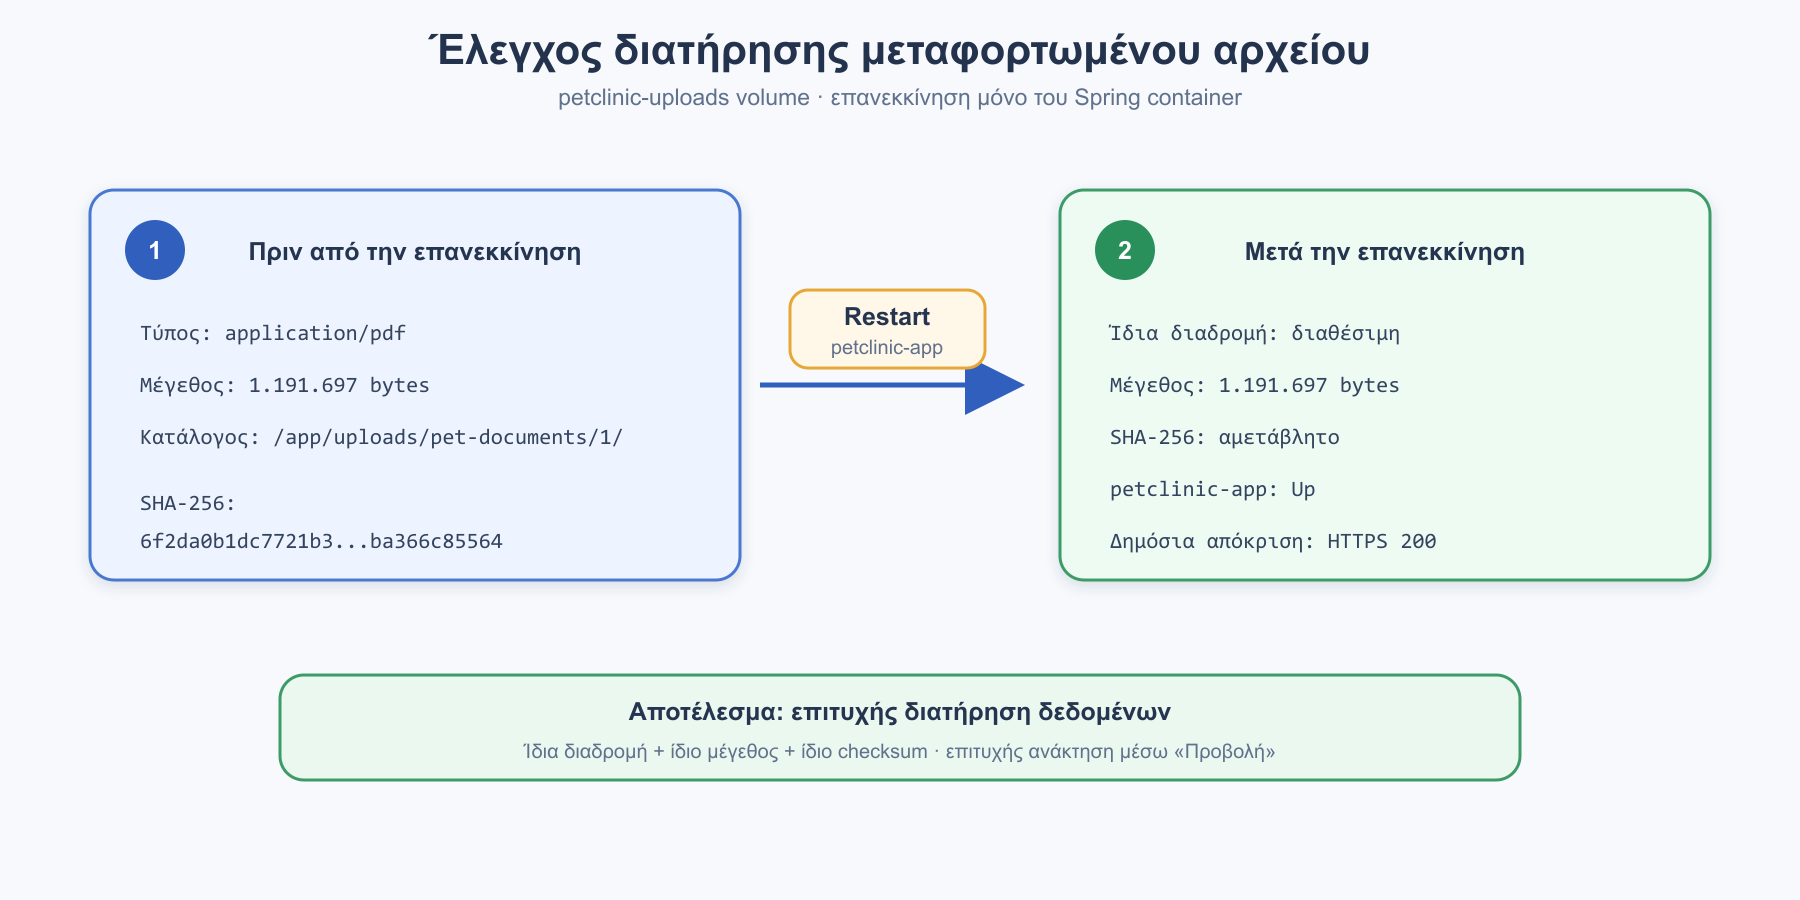
\includegraphics[width=\textwidth]{figures/infrastructure/upload-volume-persistence.png}
\caption{Επαλήθευση του persistent upload volume πριν και μετά την
επανεκκίνηση του Spring container. Η ταυτότητα του αρχείου επιβεβαιώνεται με
διαδρομή, μέγεθος και checksum, ενώ η ανάκτηση ελέγχεται από την εφαρμογή.}
\label{fig:upload-persistence-evaluation}
\end{figure}

Κατά την ίδια εκκίνηση το Liquibase ανέγνωσε τέσσερα changesets ως ήδη
εκτελεσμένα, δεν εκτέλεσε νέα μεταβολή και αποδέσμευσε επιτυχώς το changelog
lock. Το αποτέλεσμα αποτελεί ένδειξη επαναλήψιμης εκκίνησης χωρίς αυθαίρετη
τροποποίηση του schema. Δεν ισοδυναμεί όμως με πλήρη δοκιμή καταστροφής.

Στη συνέχεια πραγματοποιήθηκε ελεγχόμενο reboot ολόκληρου του EC2 instance.
Εξωτερικός watcher έλεγχε επαναληπτικά το δημόσιο HTTPS endpoint, ώστε η
μέτρηση να μην εξαρτάται από το ίδιο το instance. Η επανεκκίνηση ζητήθηκε στις
17:33:01~UTC. Η πρώτη αποτυχία καταγράφηκε στις 17:33:02,588~UTC και η πρώτη
απάντηση HTTP~200 στις 17:33:43,377~UTC, δηλαδή παρατηρήθηκε μη διαθεσιμότητα
40,79~s. Ακολούθησαν τρεις συνεχόμενες επιτυχείς απαντήσεις. Η ακολουθία των
παρατηρήσεων ήταν αποτυχία σύνδεσης, προσωρινή απάντηση HTTP~502 κατά την
εκκίνηση του upstream και τελικά HTTP~200.

Μετά το reboot τα τρία containers επανήλθαν αυτόματα μέσω πολιτικής
\texttt{unless-stopped}: το MySQL container ήταν \texttt{healthy} και τα
Spring και Nginx containers σε κατάσταση \texttt{Up}. Η εφαρμογή ολοκλήρωσε
την εκκίνησή της σε 18,352~s. Το αναπτυγμένο JAR διατήρησε το SHA-256
\texttt{317132aeac05f139\ldots de2153c82f3}, ενώ το δοκιμαστικό PDF διατήρησε
τόσο το μέγεθος 1.191.697 bytes όσο και το πλήρες checksum της προηγούμενης
μέτρησης. Τέλος, οι πληθικότητες των πινάκων ιδιοκτητών, κατοικιδίων, ραντεβού
και χρηστών παρέμειναν αντίστοιχα 2, 2, 2 και 3. Επομένως, στην ελεγχόμενη αυτή
δοκιμή επιβεβαιώθηκαν η αυτόματη επαναφορά των services και η διατήρηση βάσης
και uploads. Το αποτέλεσμα δεν αποτελεί απόδειξη υψηλής διαθεσιμότητας,
καθώς κατά το reboot υπήρξε αναμενόμενο διάστημα διακοπής.

\section{Έλεγχοι ασφάλειας}
Οι έλεγχοι που έχουν ήδη καταγραφεί επιβεβαιώνουν την ανακατεύθυνση HTTP σε
HTTPS, την απόρριψη λανθασμένων credentials και την απαγόρευση σύνδεσης σε
επιβεβαιωμένο αλλά μη εγκεκριμένο λογαριασμό. Οι διοικητικές λειτουργίες
εκτελέστηκαν από λογαριασμό με κατάλληλο ρόλο, ενώ τα tokens verification και
password reset αποθηκεύονται ως SHA-256 hashes και έχουν περιορισμένη διάρκεια
ζωής. Στις μεταφορτώσεις εφαρμόζεται όριο 10~MB και έλεγχος κανονικοποιημένης
διαδρομής ώστε το τελικό path να παραμένει εντός του upload root.

Στις 5 Σεπτεμβρίου 2026 εκτελέστηκε επαναλήψιμο σύνολο δέκα ελέγχων HTTP στην
παραγωγική εγκατάσταση. Οι δημόσιες σελίδες αρχικής και σύνδεσης επέστρεψαν
HTTP~200. Χωρίς authentication, τα endpoints dashboard, owners και
administration επέστρεψαν HTTP~401, ενώ η προσπάθεια σύνδεσης με λανθασμένο
κωδικό επέστρεψε επίσης HTTP~401. Μετά από έγκυρη σύνδεση συνθετικού χρήστη
με αποκλειστικό ρόλο \texttt{STAFF}, τα endpoints ταυτότητας και ανάγνωσης
owners επέστρεψαν HTTP~200, αλλά το διοικητικό endpoint επέστρεψε HTTP~403.
Όλοι οι αναμενόμενοι κωδικοί επιβεβαιώθηκαν, χωρίς να αποθηκευτούν
credentials, JWT ή response bodies στο τεκμήριο.

Εκτελέστηκε επίσης αρνητικός έλεγχος του ορίου μεταφόρτωσης. Συνθετικό αρχείο
10.485.761 bytes, δηλαδή ένα byte πάνω από το δηλωμένο όριο των 10~MiB,
υποβλήθηκε από τον ίδιο authenticated χρήστη και απορρίφθηκε με HTTP~413.
Μετά την απόρριψη επιβεβαιώθηκαν μηδενική νέα εγγραφή με τον δοκιμαστικό τίτλο
στον πίνακα \texttt{pet\_health\_records} και μηδενικό αντίστοιχο αρχείο στο
persistent upload volume. Το προσωρινό τοπικό payload διαγράφηκε.

Η επισκόπηση του κώδικα έδειξε ότι η τρέχουσα έκδοση περιορίζει το μέγεθος και
την τελική διαδρομή, αλλά δεν εφαρμόζει allowlist τύπων MIME ή επεκτάσεων.
Επομένως δεν παρουσιάζεται ανύπαρκτος έλεγχος \enquote{μη επιτρεπτού τύπου}
ως επιτυχής· η προσθήκη allowlist καταγράφεται ως πρόταση σκλήρυνσης. Για την
ολοκλήρωση της σκλήρυνσης προτείνεται ο συνδυασμός allowlist, ελέγχου
πραγματικού περιεχομένου και αποθήκευσης εκτός web root.

Ο έλεγχος εξαρτήσεων εκτελέστηκε σε δύο επίπεδα. Το \texttt{npm audit}, το
οποίο αντιπαραβάλλει το dependency tree του lockfile με τα advisories του
registry \cite{npm2026audit}, ανέφερε για τις 64 production frontend
dependencies δύο ευάλωτα packages υψηλής σοβαρότητας:
\texttt{react-router-dom} ως άμεση εξάρτηση και \texttt{react-router} ως
μεταβατική, με διαθέσιμη διόρθωση. Όταν συμπεριλήφθηκαν και οι build-time
εξαρτήσεις, αναφέρθηκαν 15 packages συνολικά: 12 υψηλής, 2 μέτριας και 1
χαμηλής σοβαρότητας. Ο διαχωρισμός είναι σημαντικός, επειδή εργαλεία όπως
Vite και ESLint χρησιμοποιούνται κατά το build και δεν εκτελούνται ως Node
services στην παραγωγή.

Παράλληλα, το ακριβές deployed Docker image
\texttt{sha256:1b1a0980\ldots ba47835e} σαρώθηκε με Trivy~0.73.0, το οποίο
αναλύει τόσο OS packages όσο και βιβλιοθήκες εφαρμογής σε container images
\cite{aquasecurity2026trivyimage}. Καταγράφηκαν 250 advisory matches: 9
critical, 34 high, 160 medium και 47 low. Η κατανομή ήταν 161 low/medium
ευρήματα στο Ubuntu base layer, 81 στη Java layer και 8 high στο βοηθητικό
binary \texttt{pebble}. Και τα 9 critical ευρήματα βρίσκονταν στη Java layer,
κυρίως στις παλαιότερες εκδόσεις embedded Tomcat και Spring Security που
κληρονομούνται από το Spring Boot~3.2.8. Η ενδεδειγμένη αποκατάσταση είναι
αναβάθμιση του Spring Boot dependency train και του React Router, επιλογή
ενημερωμένου και μικρότερου runtime base image, rebuild και επανάληψη των
regression/security tests.

Τα παραπάνω αποτελέσματα αποτελούν αντιστοιχίσεις αυτοματοποιημένων βάσεων
advisories και όχι απόδειξη ότι κάθε CVE είναι εκμεταλλεύσιμο στη συγκεκριμένη
διαμόρφωση. Απαιτείται triage ως προς τη χρησιμοποιούμενη λειτουργία, τις
προϋποθέσεις κάθε CVE και την πραγματική προσβασιμότητα. Ωστόσο, η ύπαρξη
διαθέσιμων fixed versions, ιδιαίτερα για critical runtime components,
καθιστά την αναβάθμιση απαραίτητο βήμα πριν από χρήση πέρα από το πλαίσιο της
διπλωματικής επίδειξης.

Η τελική μέτρηση TLS έδειξε ότι το Nginx επιτρέπει αποκλειστικά TLS~1.2 και
TLS~1.3· και οι δύο εκδόσεις διαπραγματεύτηκαν επιτυχώς με AEAD cipher suites.
Το πιστοποιητικό Let's Encrypt είχε subject
\texttt{CN=thesis-tasiopoulos.com}, κάλυπτε επιπλέον το
\texttt{www.thesis-tasiopoulos.com} και ήταν έγκυρο από 31 Αυγούστου έως 29
Νοεμβρίου 2026. Το HTTP endpoint επέστρεψε 301, το HTTPS endpoint 200 και
παρατηρήθηκε ο header \path{Strict-Transport-Security}, με διάρκεια ενός
έτους και την οδηγία \path{includeSubDomains}. Καταγράφηκαν επίσης ο
\path{X-Content-Type-Options} με τιμή \path{nosniff} και Content
Security Policy που περιορίζει το \path{frame-ancestors} στα δύο ονόματα
του domain.

\section{Οικονομική αξιολόγηση}
Η CloudFront distribution εντάχθηκε στο Free flat-rate plan, για το οποίο η
κονσόλα εμφάνισε \texttt{\$0/month} και εκτιμώμενη χρέωση ημέρας
\texttt{\$0}. Το plan περιλαμβάνει συγκεκριμένα μηνιαία όρια χρήσης και δεν
χρεώνει υπερβάσεις, σύμφωνα με την τεκμηρίωση της AWS
\cite{aws2026cloudfrontplans}. Η παρατήρηση αφορά αποκλειστικά τη χρέωση του
CloudFront plan και δεν αναιρεί πιθανές χρεώσεις της προϋπάρχουσας υποδομής.

Στις 7 Σεπτεμβρίου 2026, μετά την καθυστερημένη ενημέρωση των στοιχείων
χρέωσης, το Cost Explorer ρυθμίστηκε με net unblended cost, εξαίρεση refunds
και credits και ομαδοποίηση ανά υπηρεσία. Για τον τρέχοντα κύκλο του
Σεπτεμβρίου εμφάνισε εκτιμώμενο κόστος κατανάλωσης \texttt{\$5.38}. Η
πρόβλεψη της AWS για το τέλος του μήνα ήταν \texttt{\$9.59}, εφόσον
διατηρούνταν αντίστοιχο μοτίβο χρήσης, ενώ το συνολικό κόστος του Αυγούστου
ήταν \texttt{\$1.04}. Οι τιμές του τρέχοντος billing period παραμένουν
προσωρινές: το Cost Explorer ανανεώνει τα δεδομένα τουλάχιστον μία φορά ανά
24 ώρες και μπορεί να διαφέρει προσωρινά από τη σελίδα Bills λόγω χρόνου
ενημέρωσης και στρογγυλοποίησης
\cite{aws2026costexplorer,aws2026billingdifferences}.

Ο Πίνακας~\ref{tab:aws-observed-costs} παρουσιάζει την κατανομή του
καταγεγραμμένου κόστους. Το EC2 compute ήταν ο κυρίαρχος παράγοντας με
\texttt{\$3.51}, περίπου 65,2\% του συνόλου. Ακολουθούσαν το VPC με
\texttt{\$0.74}, το EC2--Other με \texttt{\$0.62} και το Route~53 με
\texttt{\$0.50}. Οι επιμέρους τιμές δεν αθροίζουν ακριβώς στο εμφανιζόμενο
σύνολο λόγω στρογγυλοποίησης σε δύο δεκαδικά ψηφία.

\begin{table}[htbp]
\centering
\caption{Παρατηρημένο κόστος AWS για τον Σεπτέμβριο έως 7/9/2026.}
\label{tab:aws-observed-costs}
\small
\begin{tabularx}{0.92\textwidth}{Xrr}
\toprule
Υπηρεσία & Κόστος (USD) & Μερίδιο συνόλου \\
\midrule
EC2 compute & \texttt{\$3.51} & 65,2\% \\
VPC & \texttt{\$0.74} & 13,8\% \\
EC2--Other & \texttt{\$0.62} & 11,5\% \\
Route~53 & \texttt{\$0.50} & 9,3\% \\
SES, S3, CloudWatch, CloudFront, KMS, Glue και CloudShell & \texttt{\$0.00} ανά υπηρεσία & $<$0,1\% \\
\midrule
Σύνολο Cost Explorer & \texttt{\$5.38} & 100\% \\
\bottomrule
\end{tabularx}
\end{table}

Η σελίδα Bills εμφάνιζε ταυτόχρονα εκτιμώμενο πληρωτέο ποσό
\texttt{\$0.00}, επειδή ενεργές προωθητικές πιστώσεις κάλυπταν την
κατανάλωση. Επομένως διακρίνονται δύο διαφορετικά μεγέθη: το κόστος των
πόρων που κατανάλωσε η εγκατάσταση και το ποσό που τελικά επιβαρύνει τον
χρήστη μετά την εφαρμογή πιστώσεων. Οι πιστώσεις αποτελούν προσωρινό όφελος
του συγκεκριμένου λογαριασμού και δεν χρησιμοποιούνται ως βάση για την
εκτίμηση του κανονικού λειτουργικού κόστους. Με τα δεδομένα της παρατήρησης,
η πειραματική λειτουργία αντιστοιχεί σε τάξη μεγέθους περίπου
\texttt{\$9--10} ανά μήνα, όχι σε μηδενικό οικονομικό κόστος.

Ξεχωριστά από το CloudFront Free plan, το πρόγραμμα AWS Free Tier για νέους
πελάτες προβλέπει αρχική πίστωση και δυνατότητα απόκτησης πρόσθετων πιστώσεων
με την ολοκλήρωση εκπαιδευτικών δραστηριοτήτων που εμφανίζονται στο
\enquote{Explore AWS}, όπως η εκκίνηση EC2 instance ή η δημιουργία budget.
Οι πιστώσεις αυτές είναι προσωρινές και καλύπτουν επιλέξιμες χρεώσεις· δεν
μετατρέπουν την πραγματική κατανάλωση πόρων σε μηδενικό κόστος
\cite{aws2026freetieractivities}.

Ο Πίνακας~\ref{tab:aws-cost-drivers} συνοψίζει τα στοιχεία που θα
δημιουργούσαν χρέωση χωρίς πιστώσεις. Οι τιμές είναι τιμές καταλόγου χωρίς
φόρους και όχι δεσμευτική προσφορά· η τελική χρέωση εξαρτάται από τις ώρες
λειτουργίας, την κίνηση και την ισχύ των εκάστοτε Free Tier παροχών.

\begin{table}[htbp]
\centering
\caption{Κύριοι παράγοντες κόστους της πειραματικής εγκατάστασης.}
\label{tab:aws-cost-drivers}
\small
\begin{tabularx}{\textwidth}{p{0.19\textwidth}p{0.31\textwidth}X}
\toprule
Υπηρεσία & Μονάδα χρέωσης & Εφαρμογή στην εγκατάσταση \\
\midrule
EC2 & Χρόνος λειτουργίας του instance, ανά δευτερόλεπτο με ελάχιστο 60~s & Το \texttt{t3.small} είναι ο βασικός επαναλαμβανόμενος υπολογιστικός πόρος· η χρέωση compute σταματά όταν το instance σταματήσει \cite{aws2026ec2pricing}. \\
EBS & Provisioned GB ανά μήνα & Το volume \texttt{gp3} των 30~GiB συνεχίζει να χρεώνεται όσο παραμένει δεσμευμένο, ακόμη και με σταματημένο EC2· τα βασικά 3.000 IOPS και 125~MB/s περιλαμβάνονται \cite{aws2026ebspricing}. \\
Public IPv4 & \texttt{\$0.005} ανά διεύθυνση και ώρα & Μία διεύθυνση επί 30 ημέρες αντιστοιχεί περίπου σε \texttt{\$3.60}, είτε είναι σε χρήση είτε παραμένει δεσμευμένη \cite{aws2026vpcpricing}. \\
Route~53 & \texttt{\$0.50} ανά hosted zone τον μήνα και \texttt{\$0.40}/εκατ. standard queries & Η κατοχύρωση του \texttt{.com} χρεώνεται χωριστά σε ετήσια βάση· το χαμηλό πειραματικό DNS traffic είναι πρακτικά αμελητέο \cite{aws2026route53pricing}. \\
SES & \texttt{\$0.10}/1.000 outbound emails και \texttt{\$0.12}/GB εξερχόμενων δεδομένων & Οι λίγες staff verification και password-reset αποστολές έχουν κόστος πολύ μικρότερο του ενός cent· δεν χρησιμοποιήθηκαν dedicated IPs \cite{aws2026sespricing}. \\
CloudWatch & Βασικά service metrics χωρίς πρόσθετη χρέωση· detailed/custom metrics και logs με χρέωση & Χρησιμοποιήθηκαν μόνο τα προεπιλεγμένα πεντάλεπτα EC2 metrics και status checks, χωρίς Agent ή log ingestion \cite{aws2026cloudwatchbasic}. \\
S3 & Αποθήκευση, requests και μεταφορά δεδομένων & Το προσωρινό deployment object περίπου 70,5~MB δημιουργεί αμελητέα αποθήκευση και ελάχιστα requests· η εισερχόμενη μεταφορά και η μεταφορά προς υπηρεσία στην ίδια περιοχή δεν χρεώνονται \cite{aws2026s3pricing}. \\
CloudFront & Free flat-rate plan: \texttt{\$0/month} & Περιλαμβάνει έως 1 εκατ. requests και 100~GB transfer τον μήνα χωρίς overage charge, όρια κατά πολύ μεγαλύτερα από το PoC \cite{aws2026cloudfrontplans}. \\
\bottomrule
\end{tabularx}
\end{table}

Η ανάλυση διαχωρίζει EC2, EBS, Route~53, data transfer, SES και CloudWatch,
ώστε να μην αποδίδεται ολόκληρο το κόστος σε μία μόνο υπηρεσία. Για τη
συσχέτιση των πειραμάτων χρησιμοποιήθηκαν μόνο τα βασικά EC2 metrics και τα
status checks. Δεν εγκαταστάθηκε CloudWatch Agent και δεν δημιουργήθηκαν
custom metrics ή πρόσθετη συλλογή logs, συνεπώς η αξιολόγηση δεν εισήγαγε
τέτοια πρόσθετη χρέωση. Ως προληπτικό μέτρο προετοιμάστηκε AWS Budget
μηδενικής δαπάνης, με προτεινόμενη ειδοποίηση όταν η καταγεγραμμένη δαπάνη
υπερβεί τα \texttt{\$0.01}. Η ενεργοποίηση της ειδοποίησης δεν αποτελεί
μέρος της μέτρησης και μπορεί να γίνει πριν παραμείνει η υποδομή ενεργή για
μεγαλύτερο διάστημα. Δεν παρουσιάζονται account identifiers, διευθύνσεις
ειδοποίησης ή στοιχεία πληρωμής.

\section{Συζήτηση αποτελεσμάτων και περιορισμών}
Τα έως τώρα αποτελέσματα δείχνουν ότι η μονοκομβική containerized εγκατάσταση
είναι λειτουργική, χρησιμοποιεί έγκυρο HTTPS, εκτελεί επαναλήψιμες migrations
και διατηρεί μεταφορτωμένα δεδομένα όταν αντικαθίσταται ή επανεκκινείται το
application container. Η επιτυχής ανάκτηση του PDF από τη διεπαφή είναι
ισχυρότερη ένδειξη από την απλή ύπαρξη του αρχείου στο filesystem, επειδή
ελέγχει ταυτόχρονα metadata, backend endpoint και browser flow.

Τα ευρήματα δεν αποδεικνύουν υψηλή διαθεσιμότητα. Υπάρχει ένα EC2 instance,
μία MySQL και ένα application container, χωρίς load balancer ή δεύτερη ζώνη
διαθεσιμότητας. Το reboot επιβεβαίωσε την αυτόματη επαναφορά, αλλά κατέγραψε
διακοπή 40,79~s και δεν υποκαθιστά δοκιμή restore από backup ή αστοχία
ολόκληρης ζώνης διαθεσιμότητας. Οι περιορισμοί αυτοί παραμένουν ρητοί κατά
την ερμηνεία των load, stress, soak και cost results.

\section{Κατάλογος ολοκληρωμένων ελέγχων και τεκμηρίων}
Ο Πίνακας~\ref{tab:evaluation-status} λειτουργεί ως συνοπτικός χάρτης των
ελέγχων που παρουσιάστηκαν αναλυτικά στις προηγούμενες ενότητες. Δεν
αποτελεί εσωτερικό πίνακα παρακολούθησης εργασιών: καταγράφει το αντικείμενο
κάθε δοκιμής, το παρατηρηθέν αποτέλεσμα και το τεκμήριο στο οποίο βασίζεται,
ώστε ο αναγνώστης να μπορεί να εντοπίσει γρήγορα το εύρος της αξιολόγησης.

\begin{table}[htbp]
\centering
\caption{Κατάλογος ολοκληρωμένων ελέγχων και κύριων τεκμηρίων.}
\label{tab:evaluation-status}
\small
\begin{tabularx}{\textwidth}{p{0.34\textwidth}p{0.20\textwidth}X}
\toprule
Αντικείμενο ελέγχου & Αποτέλεσμα & Κύριο τεκμήριο \\
\midrule
Λειτουργικές ροές και SES & Επιτυχία & Εγγραφή, verification, approval και reset \\
DNS, HTTP και HTTPS & Επιτυχία & DNS resolution, 301 redirect και HTTPS 200 \\
Liquibase restart & Επιτυχία & 4 previously run, 0 νέα changesets \\
Upload και προβολή PDF & Επιτυχία & Metadata και επιτυχής ανάκτηση στον browser \\
Persistence μετά από app restart & Επιτυχία & Ίδιο path, μέγεθος και SHA-256 \\
CloudFront proof of concept & Επιτυχία & Free plan, HTTPS origin, HTTP redirect, αρχική σελίδα και \texttt{/login} \\
Response-time baseline & Επιτυχία & 895 αιτήματα, 14,91 requests/s και 0 σφάλματα \\
Load stages 1/5/10/25 VU & Επιτυχία με εμφανές όριο & 0 σφάλματα έως 339,73 requests/s και υποβάθμιση login \\
Stress/soak & Επιτυχία & Stop point στα 25 VU και 5 VU για 300~s χωρίς σφάλματα \\
CloudWatch correlation & Επιτυχία & CPU, network και status checks για baseline, load και soak \\
EC2 reboot & Επιτυχία με μετρημένη διακοπή & Αυτόματη επαναφορά, persistence και HTTPS σε 40,79~s \\
Security matrix & Επιτυχία εντός πεδίου & API/RBAC, όριο upload, dependency scan και TLS \\
Πραγματικό κόστος & Καταγράφηκε & Cost Explorer, Bills, credits και τιμές καταλόγου ανά υπηρεσία \\
\bottomrule
\end{tabularx}
\end{table}
